% Options for packages loaded elsewhere
\PassOptionsToPackage{unicode}{hyperref}
\PassOptionsToPackage{hyphens}{url}
\PassOptionsToPackage{dvipsnames,svgnames,x11names}{xcolor}
%
\documentclass[
  letterpaper,
  DIV=11,
  numbers=noendperiod]{scrreprt}

\usepackage{amsmath,amssymb}
\usepackage{iftex}
\ifPDFTeX
  \usepackage[T1]{fontenc}
  \usepackage[utf8]{inputenc}
  \usepackage{textcomp} % provide euro and other symbols
\else % if luatex or xetex
  \usepackage{unicode-math}
  \defaultfontfeatures{Scale=MatchLowercase}
  \defaultfontfeatures[\rmfamily]{Ligatures=TeX,Scale=1}
\fi
\usepackage{lmodern}
\ifPDFTeX\else  
    % xetex/luatex font selection
\fi
% Use upquote if available, for straight quotes in verbatim environments
\IfFileExists{upquote.sty}{\usepackage{upquote}}{}
\IfFileExists{microtype.sty}{% use microtype if available
  \usepackage[]{microtype}
  \UseMicrotypeSet[protrusion]{basicmath} % disable protrusion for tt fonts
}{}
\makeatletter
\@ifundefined{KOMAClassName}{% if non-KOMA class
  \IfFileExists{parskip.sty}{%
    \usepackage{parskip}
  }{% else
    \setlength{\parindent}{0pt}
    \setlength{\parskip}{6pt plus 2pt minus 1pt}}
}{% if KOMA class
  \KOMAoptions{parskip=half}}
\makeatother
\usepackage{xcolor}
\setlength{\emergencystretch}{3em} % prevent overfull lines
\setcounter{secnumdepth}{5}
% Make \paragraph and \subparagraph free-standing
\ifx\paragraph\undefined\else
  \let\oldparagraph\paragraph
  \renewcommand{\paragraph}[1]{\oldparagraph{#1}\mbox{}}
\fi
\ifx\subparagraph\undefined\else
  \let\oldsubparagraph\subparagraph
  \renewcommand{\subparagraph}[1]{\oldsubparagraph{#1}\mbox{}}
\fi


\providecommand{\tightlist}{%
  \setlength{\itemsep}{0pt}\setlength{\parskip}{0pt}}\usepackage{longtable,booktabs,array}
\usepackage{calc} % for calculating minipage widths
% Correct order of tables after \paragraph or \subparagraph
\usepackage{etoolbox}
\makeatletter
\patchcmd\longtable{\par}{\if@noskipsec\mbox{}\fi\par}{}{}
\makeatother
% Allow footnotes in longtable head/foot
\IfFileExists{footnotehyper.sty}{\usepackage{footnotehyper}}{\usepackage{footnote}}
\makesavenoteenv{longtable}
\usepackage{graphicx}
\makeatletter
\def\maxwidth{\ifdim\Gin@nat@width>\linewidth\linewidth\else\Gin@nat@width\fi}
\def\maxheight{\ifdim\Gin@nat@height>\textheight\textheight\else\Gin@nat@height\fi}
\makeatother
% Scale images if necessary, so that they will not overflow the page
% margins by default, and it is still possible to overwrite the defaults
% using explicit options in \includegraphics[width, height, ...]{}
\setkeys{Gin}{width=\maxwidth,height=\maxheight,keepaspectratio}
% Set default figure placement to htbp
\makeatletter
\def\fps@figure{htbp}
\makeatother
% definitions for citeproc citations
\NewDocumentCommand\citeproctext{}{}
\NewDocumentCommand\citeproc{mm}{%
  \begingroup\def\citeproctext{#2}\cite{#1}\endgroup}
\makeatletter
 % allow citations to break across lines
 \let\@cite@ofmt\@firstofone
 % avoid brackets around text for \cite:
 \def\@biblabel#1{}
 \def\@cite#1#2{{#1\if@tempswa , #2\fi}}
\makeatother
\newlength{\cslhangindent}
\setlength{\cslhangindent}{1.5em}
\newlength{\csllabelwidth}
\setlength{\csllabelwidth}{3em}
\newenvironment{CSLReferences}[2] % #1 hanging-indent, #2 entry-spacing
 {\begin{list}{}{%
  \setlength{\itemindent}{0pt}
  \setlength{\leftmargin}{0pt}
  \setlength{\parsep}{0pt}
  % turn on hanging indent if param 1 is 1
  \ifodd #1
   \setlength{\leftmargin}{\cslhangindent}
   \setlength{\itemindent}{-1\cslhangindent}
  \fi
  % set entry spacing
  \setlength{\itemsep}{#2\baselineskip}}}
 {\end{list}}
\usepackage{calc}
\newcommand{\CSLBlock}[1]{\hfill\break\parbox[t]{\linewidth}{\strut\ignorespaces#1\strut}}
\newcommand{\CSLLeftMargin}[1]{\parbox[t]{\csllabelwidth}{\strut#1\strut}}
\newcommand{\CSLRightInline}[1]{\parbox[t]{\linewidth - \csllabelwidth}{\strut#1\strut}}
\newcommand{\CSLIndent}[1]{\hspace{\cslhangindent}#1}

\KOMAoption{captions}{tableheading}
\makeatletter
\@ifpackageloaded{bookmark}{}{\usepackage{bookmark}}
\makeatother
\makeatletter
\@ifpackageloaded{caption}{}{\usepackage{caption}}
\AtBeginDocument{%
\ifdefined\contentsname
  \renewcommand*\contentsname{Table of contents}
\else
  \newcommand\contentsname{Table of contents}
\fi
\ifdefined\listfigurename
  \renewcommand*\listfigurename{List of Figures}
\else
  \newcommand\listfigurename{List of Figures}
\fi
\ifdefined\listtablename
  \renewcommand*\listtablename{List of Tables}
\else
  \newcommand\listtablename{List of Tables}
\fi
\ifdefined\figurename
  \renewcommand*\figurename{Figure}
\else
  \newcommand\figurename{Figure}
\fi
\ifdefined\tablename
  \renewcommand*\tablename{Table}
\else
  \newcommand\tablename{Table}
\fi
}
\@ifpackageloaded{float}{}{\usepackage{float}}
\floatstyle{ruled}
\@ifundefined{c@chapter}{\newfloat{codelisting}{h}{lop}}{\newfloat{codelisting}{h}{lop}[chapter]}
\floatname{codelisting}{Listing}
\newcommand*\listoflistings{\listof{codelisting}{List of Listings}}
\makeatother
\makeatletter
\makeatother
\makeatletter
\@ifpackageloaded{caption}{}{\usepackage{caption}}
\@ifpackageloaded{subcaption}{}{\usepackage{subcaption}}
\makeatother
\ifLuaTeX
  \usepackage{selnolig}  % disable illegal ligatures
\fi
\usepackage{bookmark}

\IfFileExists{xurl.sty}{\usepackage{xurl}}{} % add URL line breaks if available
\urlstyle{same} % disable monospaced font for URLs
\hypersetup{
  pdftitle={Fuerzas: Fichas},
  pdfauthor={David Domínguez Román},
  colorlinks=true,
  linkcolor={blue},
  filecolor={Maroon},
  citecolor={Blue},
  urlcolor={Blue},
  pdfcreator={LaTeX via pandoc}}

\title{Fuerzas: Fichas}
\author{David Domínguez Román}
\date{2024-04-01}

\begin{document}
\maketitle

\renewcommand*\contentsname{Table of contents}
{
\hypersetup{linkcolor=}
\setcounter{tocdepth}{2}
\tableofcontents
}
\bookmarksetup{startatroot}

\chapter*{Preface}\label{preface}
\addcontentsline{toc}{chapter}{Preface}

\markboth{Preface}{Preface}

This is a Quarto book.

To learn more about Quarto books visit
\url{https://quarto.org/docs/books}.

\bookmarksetup{startatroot}

\chapter{Introduction}\label{introduction}

This is a book created from markdown and executable code.

See Knuth (1984) for additional discussion of literate programming.

\bookmarksetup{startatroot}

\chapter{Fuerzas: tipos de fuerzas, tipos de cuerpos y Ley de
Hook}\label{fuerzas-tipos-de-fuerzas-tipos-de-cuerpos-y-ley-de-hook}

Nombre:\_\_\_\_\_\_\_\_\_\_\_\_\_\_\_\_\_\_\_\_\_\_\_\_\_\_\_\_\_\_\_\_\_\_\_\_\_\_\_\_\_\_\_\_\_\_\_\_\_\_\_\_\_\_\_\_\_\_\_\_\_\_\_\_\_\_\_\_\_\_\_\_\_\_\_\_\_\_

\begin{center}\rule{0.5\linewidth}{0.5pt}\end{center}

\begin{center}\rule{0.5\linewidth}{0.5pt}\end{center}

Una \textbf{fuerza} es toda causa que pueda deformar un objeto o
modificar su estado de reposo o movimiento. La unidad de fuerza en el
Sistema Internacional es el Newton (N).

Los \textbf{efectos} de una fuerza son:

\begin{itemize}
\tightlist
\item
  Poder \textbf{mover un cuerpo} que estaba parado.
\item
  Poder \textbf{parar un cuerpo} que se estaba moviendo.
\item
  Poder \textbf{modificar la velocidad} de un objeto.
\item
  Poder producir \textbf{deformaciones}.
\end{itemize}

Las fuerzas pueden actuar de distintas \textbf{formas}:

\begin{itemize}
\item
  \textbf{Por contacto}: por ejemplo, al empujar una silla o golpear un
  balón.
\item
  \textbf{A distancia}: no es necesario que haya un contacto físico
  entre los cuerpos.

  \begin{itemize}
  \tightlist
  \item
    Gravitatoria.
  \item
    Magnética.
  \item
    Eléctrica.
  \end{itemize}
\end{itemize}

\begin{center}\rule{0.5\linewidth}{0.5pt}\end{center}

\begin{center}\rule{0.5\linewidth}{0.5pt}\end{center}

\textbf{1.-} Una \_\_\_\_\_\_ es todo aquello que puede
\_\_\_\_\_\_\_\_\_ un objeto y/o \_\_\_\_\_\_\_\_ su estado de reposo o
movimiento. Puede \_\_\_\_\_\_\_ un objeto parado, \_\_\_\_\_\_ un
objeto en \_\_\_\_\_\_\_, modificar su \_\_\_\_\_\_\_\_ o producir
\_\_\_\_\_\_\_\_\_\_.

\begin{longtable}[]{@{}ccc@{}}
\toprule\noalign{}
\endhead
\bottomrule\noalign{}
\endlastfoot
parar & deformar & deformaciones \\
mover & fuerza & modificar \\
velocidad & & \\
\end{longtable}

\textbf{2.-} Indica si las siguientes fuerzas actúan \textbf{por
contacto} o \textbf{a distancia}:

\begin{itemize}
\item
  Alexia Putellas lanza un penalti:
\item
  Fernando Alonso acelera al comienzo de la carrera:
\item
  Un imán en la nevera:
\item
  Un electrón gira alrededor de un núcleo atómico:
\item
  La Luna orbita la Tierra:
\item
  Un imán atrae una barra de hierro:
\item
  Un barco se detiene:
\item
  Un avión ha despegado y coge velocidad:
\item
  Un avión asciende:
\item
  Al frotar una regla contra lana, esta atrae trocitos de papel:
\end{itemize}

\textbf{3.-} Cita \textbf{tres acciones} de la vida cotidiana en la que
se produzca:

\begin{itemize}
\item
  Una deformación de un cuerpo:
\item
  El movimiento de un cuerpo que estaba en reposo:
\item
  El cambio de movimiento de un cuerpo (acelerar, desacelerar o cambiar
  la dirección):
\end{itemize}

\textbf{4.-} ¿ De qué \textbf{forma} actúa la fuerza de atracción entre
un protón y un electrón?

\begin{center}\rule{0.5\linewidth}{0.5pt}\end{center}

\begin{center}\rule{0.5\linewidth}{0.5pt}\end{center}

Los \textbf{cuerpos} pueden \textbf{clasificarse} en:

\begin{longtable}[]{@{}
  >{\raggedright\arraybackslash}p{(\columnwidth - 2\tabcolsep) * \real{0.6802}}
  >{\centering\arraybackslash}p{(\columnwidth - 2\tabcolsep) * \real{0.3198}}@{}}
\toprule\noalign{}
\endhead
\bottomrule\noalign{}
\endlastfoot
\begin{minipage}[t]{\linewidth}\raggedright
\begin{itemize}
\tightlist
\item
  \textbf{Rígidos}: \textbf{no se deforman} ante la acción de una
  fuerza. Por ejemplo: la pata de una silla.
\end{itemize}
\end{minipage} &
\includegraphics[width=0.28\textwidth,height=\textheight]{D_NQ_NP_770113-MLA46490092791_062021-W.webp} \\
\begin{minipage}[t]{\linewidth}\raggedright
\begin{itemize}
\tightlist
\item
  \textbf{Plásticos}: \textbf{se deforman} bajo la acción de una fuerza,
  pero \textbf{no vuelven a su estado natural} cuando deja de actuar.
  Por ejemplo, el pan.
\end{itemize}
\end{minipage} &
\includegraphics[width=1.4375in,height=\textheight]{Little_girl_holding_plasticine._(49810941302).webp} \\
\begin{minipage}[t]{\linewidth}\raggedright
\begin{itemize}
\tightlist
\item
  \textbf{Elásticos}: son \textbf{capaces de recuperar su forma inicial}
  cuando una fuerza los ha deformado. Por ejemplo: una goma elástica.
\end{itemize}
\end{minipage} &
\includegraphics[width=1.29167in,height=\textheight]{goma-el-stica_PDT01256.webp} \\
\end{longtable}

\begin{center}\rule{0.5\linewidth}{0.5pt}\end{center}

\begin{center}\rule{0.5\linewidth}{0.5pt}\end{center}

\textbf{5.-} \textbf{Clasifica} los siguientes objetos en rígidos,
plásticos o elásticos:

\begin{itemize}
\item
  Una bola de billar:
\item
  Una goma de borrar:
\item
  Plastilina:
\item
  Un muelle:
\item
  Una esponja:
\item
  Un vaso:
\item
  El barro:
\end{itemize}

\textbf{6.-} En la industria pueden llegar a usarse muelles tan fuertes
que ni 100 elefantes pueden llegar a moverlos. Entonces\ldots. ¿Son
rígidos? \textbf{Justifica tu respuesta}. Di si son rígidos, plásticos o
elásticos y por qué.

\textbf{7.-} Una goma de borrar, si se aprieta con las manos recupera su
forma, pero si se ejerce mucha fuerza queda deformada para siempre. ¿Por
qué crees que pasa esto?

\begin{center}\rule{0.5\linewidth}{0.5pt}\end{center}

\begin{center}\rule{0.5\linewidth}{0.5pt}\end{center}

Si cogemos un muelle cualquiera y suspendemos una masa de uno de sus
extremos (la llamaremos peso), dejando el otro fijo, este se deforma y
se alarga una cantidad \(\Delta x\). Si suspendemos otra masa igual, el
muelle se alargará el doble de lo que lo había hecho. El alargamiento de
un muelle es directamente proporcional a la fuerza que se ha ejercido
para alargarlo:

\[
F = K \cdot \Delta x,
\]

siendo

\[
\Delta x = x_{final} - x_{inicial}.
\]

\(F\) es la fuerza que se ejerce y su unidad es el Newton (N), \(K\) es
la constante elástica del muelle y sus unidades son Newton por metro
(N/m) y \(x\) el alargamiento, cuyas unidades son metros (m). Un muelle
con una \(K\) más alta se alargará menos que otro con una constante
elástica más baja.

A esta ecuación la llamamos \textbf{\emph{Ley de Hooke}}.

\begin{center}
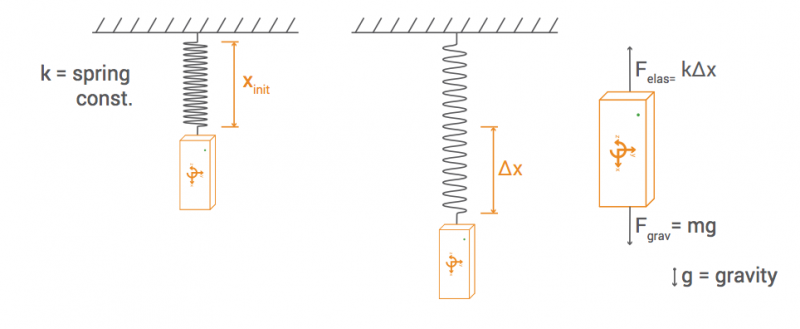
\includegraphics[width=5.94792in,height=\textheight]{Screen Shot 2017-06-01 at 12.46.01 PM.png}
\end{center}

\begin{center}
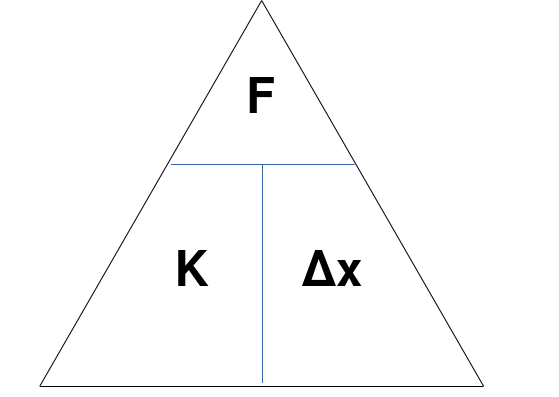
\includegraphics[width=2.97917in,height=\textheight]{Untitled 1.png}
\end{center}

\begin{center}\rule{0.5\linewidth}{0.5pt}\end{center}

\begin{center}\rule{0.5\linewidth}{0.5pt}\end{center}

\textbf{8.-} Un muelle de constante elástica \(K=20N/m\) tiene
suspendida una masa \(m=100g\). ¿Cuál será su alargamiento \(\Delta x\)?
Utiliza unidades en el \textbf{Sistema Internacional (metros, Newton,
kilogramo, etc.)}. Aceleración de la gravedad: \(g=9,8 m/s²\).

\textbf{9.-} ¿Un muelle con una longitud inicial \(x_{inicial}=20cm\) se
alarga hasta \(x_{final}=40cm\) aplicando una fuerza \(F=200N\). Calcula
la constante elástica del muelle, \(K\). Utiliza siempre unidades del
\textbf{Sistema Internacional}.

\bookmarksetup{startatroot}

\chapter{Summary}\label{summary}

In summary, this book has no content whatsoever.

\bookmarksetup{startatroot}

\chapter*{References}\label{references}
\addcontentsline{toc}{chapter}{References}

\markboth{References}{References}

\phantomsection\label{refs}
\begin{CSLReferences}{1}{0}
\bibitem[\citeproctext]{ref-knuth84}
Knuth, Donald E. 1984. {``Literate Programming.''} \emph{Comput. J.} 27
(2): 97--111. \url{https://doi.org/10.1093/comjnl/27.2.97}.

\end{CSLReferences}



\end{document}
